\chapter{Introduction and Motivation}
\label{ch:intro}


\section{Motivation}
\label{sec:motivation}


Since the discovery (and further confirmation) of the greenhouse effect in the years from 1824 to 1900 \cite{fourier1824remarques, foote1856circumstances} humans came a long way of fighting the consequences of the increased greenhouse gas concentration in earth's atmosphere. 
In 1972 \citeauthor{sawyer1972man} summarized the knwoledge and predicted quite accurately the warming at the end of the century \cite{sawyer1972man}
Especially the last decades the climate crisis gained more and more attention, leading to the creation of multiple international organizations and institutions (e.g. the International Panel on Climate Change (IPCC) in 1988).


\begin{figure}[t]
  \begin{center}
    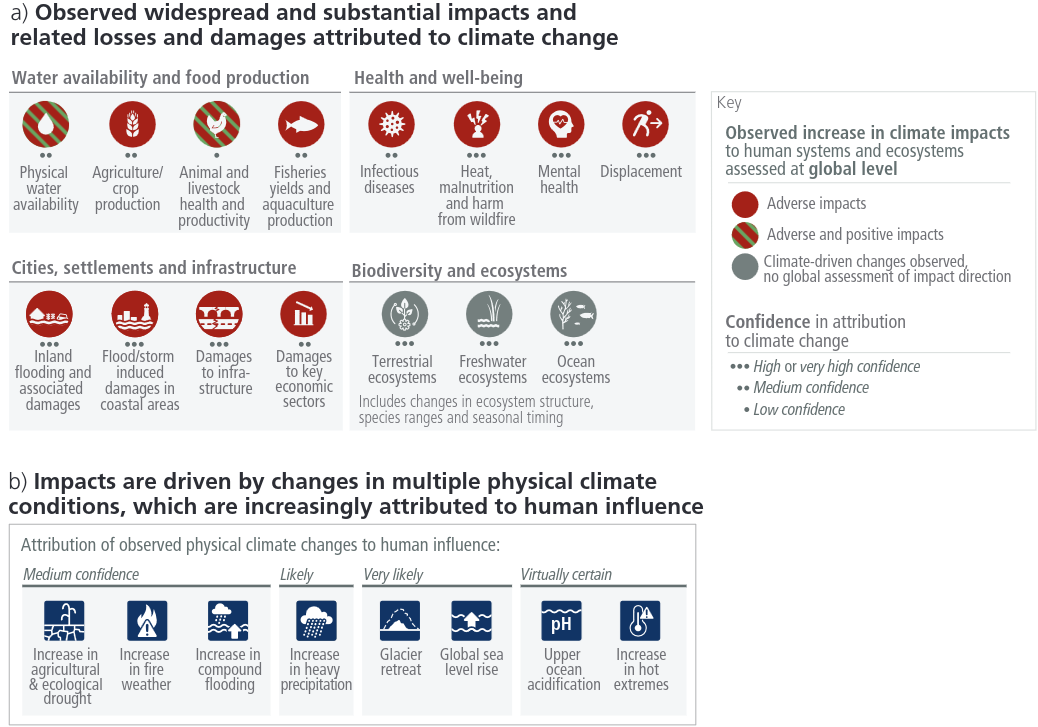
\includegraphics[width=0.95\textwidth]{figures/ipcc_6th_report_impacts_climate_change.png}
  \end{center}
  \caption{Impact of Climate Change for Humans, taken from \cite{lee2024climate}}
  \label{fig:impacts_climate_change}
\end{figure}



In 2019 more than 11,000  scientists from around the world released a declaration \cite{ripple_world_2019}, calling governments from around the world to action.
The mid and long-term consequences are manyfold and go far beyond the general rising of the worlds' average temperature (see Figure \ref{fig:impacts_climate_change}), e.g. shifts in circulation systems like the North Atlantic Oscillation (NAO) \cite{vietinghoff_visual_2021}, which in turn also have varying consequences. 
Understanding what consequences may lay ahead of us is a crucial step in tackling these challanges, and this thesis aims to follow up on the research of \citeauthor{vietinghoff_visual_2021}, trying to evaluate in a similar manner the systemic changes of moisture transport patterns in Europe and the northern Atlantic. 


\section{Climate and Climate Research}
\label{sec:climate}

This section should give an introduction to the current state of climate research. 
Therefor it should explain what the current way of future climate predictions is (Coupled Models), how they work, and 
It should explain some part of the politics, who is involed in what and what the backroud of the most important projects (CMIP, ScenarioMIP \dots). 
It should be explained that the data used is the one that the highest council of fighting climate change uses for its report. 

\begin{enumerate}
  \item
  
\end{enumerate}


\textbf{Quick overview over Climate Systems}

Contents of this section: 

\begin{itemize}
  \item What are climate systems? 
  \item What are forcings? 
  \item What does variability in climate systems stem from?
  \item 
\end{itemize}




\textbf{IPCC and the Coupled Model Intercomparison Project (CMIP)}


The reason for the endorsement of the IPCC by the UN General Assembly 1988 was to prepare comprehensive reviews and report about the current state of scientific knowledge and research. 
Since then there were six assement cycles and six reports were published, condensing the research of the scientific community. Figure \ref{fig:impacts_climate_change} is a graphic from the latest report for policy makers from 2023 \cite{lee2024climate}, displaying the probable consequences for humans in climate change.

A main source for such figures in the reports are so-called Global Coupled Models (GCMs)\footnote{Unfortunately, Global Coupled Models share their acronym with General Circulation Models, which are quite similar}, trying to model the state and evolution of certain fields of earth data.
They consist of multiple Models, each representing a major part of Earth's complex climate system (like atmosphere, hydrosphere, etc.), also allowing to model the dynamic interactions between these parts \cite{vietinghoffdiss}. 
In the mid 90s the Coupled Model Intercomparison Project (CMIP) was brought to life, with the aim of streamlining results of GCMs and making them compareable. 
CMIP provides the outer structure, amongst others what kind of simulations to produce (e.g. preindustrial control simulations, future scenarios etc.), what kinds of fields should be generated, what kind of resolutions to provide and also how these results should be serialized.
Since then the results of CMIP played an increasingly major part in the reports of the IPCC \cite{touzepeiffer_coupled_2020}, and are now even called \enquote{... one of the foundational elements of climate science} \cite{eyring_overview_2016}. 
CMIP is currently in its 6th phase, corresponding to the recently finished 6th Assessment Report of the IPCC \cite{lee2024climate}. 



\textbf{The North Atlantic Oscillation}




 
\section{Research Questions and Thesis Structure}
\label{sec:research_questions}

Following up the previous sections, the reasearch question for this thesis is: 

\begin{center}
  \larger{\enquote{How do the Patterns of Moisture Transport change in the face of various climate scenarios in the North-East Atlantic?}}
\end{center}


The remaining thesis is structured as follows: Chapter \ref{ch:basics} gives the theoretical background on fields and pattern analysis. 
The following Chapter \ref{ch:dataset} gives a detailed overview about the used CMIP6 based dataset. 
Chapter \ref{ch:related_work} provides an overview of related work, the motivation for this thesis and the placement of this thesis in the academic context. 
While the results are discussed and presented in Chapter \ref{ch:results}, Chapter \ref{ch:methodology} gives a detailed description how these results came about. 
The thesis is concluded with Chapter \ref{ch:conclusions} and gives an outlook for future research. 



% Structure:
%
% \begin{enumerate}
%   \item \textbf{Preliminaries}: explain what climate simulations are, what cmip(6) is and its relation to the IPCC reports and what that means for the global fight against the climate crisis. 
%     This chapter should prepare the reader to understand all the related work in Chapter \ref{ch:related_work}.
%   \item \textbf{Problem Analysis}: explain what I want to do using the CMIP6 simulations: Describe what the general plan is: Visualization of the moisture transport in Europe with the help. 
%     Also define what the goals of the visualizations are: Visualize different scenarios for comparison, visualize uncertainties of different members, visualize evolution over time, also try combining those. 
%     Here should be a graphic that explains the workflow that transforms a simulation into some nice pictures
%   \item \textbf{Related Work}: Show what efforts have already been done regarding analysis of moisture transport, future and past. 
%     Maybe preparing a comparison table would be good. 
%   \item \textbf{Realization}: Describe in a step by step way what measures had been taken. 
%   \item \textbf{Evaluation}: A little bit unsure how far I (as a CS person) can evaluate this, have to come up with a concept
%   \item \textbf{Conclusion}: Same as step before, but there will be something to write about after everything else is written
%   
% \end{enumerate}

